%
% Template Laporan Skripsi/Thesis 
%
% @author  Andreas Febrian, Lia Sadita 
% @version 1.03
%
% Dokumen ini dibuat berdasarkan standar IEEE dalam membuat class untuk 
% LaTeX dan konfigurasi LaTeX yang digunakan Fahrurrozi Rahman ketika 
% membuat laporan skripsi. Konfigurasi yang lama telah disesuaikan dengan 
% aturan penulisan thesis yang dikeluarkan UI pada tahun 2008.
%

%
% Tipe dokumen adalah report dengan satu kolom. 
%
\documentclass[12pt, a4paper, onecolumn, oneside, final]{report}

% Load konfigurasi LaTeX untuk tipe laporan thesis
\usepackage{_internals/uithesis}

% Load konfigurasi khusus untuk laporan yang sedang dibuat
%-----------------------------------------------------------------------------%
% Informasi Mengenai Dokumen
%-----------------------------------------------------------------------------%
%
% Judul laporan.
\var{\judul}{A Benchmarking Tool for Computational Reproducibility}
%
% Tulis kembali judul laporan, kali ini akan diubah menjadi huruf kapital
\Var{\Judul}{A Benchmarking Tool for Computational Reproducibility}
%
% Tulis kembali judul laporan namun dengan bahasa Ingris
\var{\judulInggris}{A Benchmarking Tool for Computational Reproducibility}

%
% Tipe laporan, dapat berisi Skripsi, Tugas Akhir, Thesis, atau Disertasi
\var{\type}{Thesis}
%
% Tulis kembali tipe laporan, kali ini akan diubah menjadi huruf kapital
\Var{\Type}{Thesis}

\var{\fullType}{Bachelor Thesis}
\Var{\FullType}{Bachelor Thesis}
%
% Tulis nama penulis
\var{\penulis}{Rakha Kanz Kautsar}
%
% Tulis kembali nama penulis, kali ini akan diubah menjadi huruf kapital
\Var{\Penulis}{Rakha Kanz Kautsar}
%
% Tulis NPM penulis
\var{\npm}{1506688784}
%
% Tuliskan Fakultas dimana penulis berada
\Var{\Fakultas}{Computer Science}
\var{\fakultas}{Computer Science}
%
% Tuliskan Program Studi yang diambil penulis
\Var{\Program}{Computer Science}
\var{\program}{Computer Science}
%
% Tuliskan tahun publikasi laporan
\Var{\bulan}{Juli}
\Var{\tahun}{2019}
%
% Tuliskan gelar yang akan diperoleh dengan menyerahkan laporan ini
\var{\gelar}{Bachelor of Computer Science}
%
% Tuliskan tanggal pengesahan laporan, waktu dimana laporan diserahkan ke
% penguji/sekretariat
\var{\tanggalPengesahan}{XX Juli 2019}
%
% Tuliskan tanggal keputusan sidang dikeluarkan dan penulis dinyatakan
% lulus/tidak lulus
\var{\tanggalLulus}{XX Juli 2019}
%
% Tuliskan pembimbing
\var{\pembimbing}{Drs. Lim Yohanes Stefanus, M.Math., Ph.D}
\var{\pembimbingDua}{Dr. Johannes K. Fichte}
%
% Alias untuk memudahkan alur penulisan paa saat menulis laporan
\var{\saya}{Penulis}
\var{\First}{We}
\var{\first}{we}
\var{\firstposs}{our}
\var{\Firstposs}{Our}

%-----------------------------------------------------------------------------%
% Judul Setiap Bab
%-----------------------------------------------------------------------------%
%
% Berikut ada judul-judul setiap bab.
% Silahkan diubah sesuai dengan kebutuhan.
%
\Var{\kataPengantar}{Preface}
\Var{\chIntroduction}{Introduction}
\Var{\chExperimentation}{Experimentation \& Benchmarking}
\Var{\chResource}{Measuring \& Limiting Resource}
\Var{\chExisting}{Existing Benchmarking Tools}
\Var{\chImplementation}{Implementation}
\Var{\chEvaluation}{Evaluation}
\Var{\chConclusion}{Conclusion \& Future Works}


\usetikzlibrary{shapes,arrows,positioning,fit,backgrounds}

% Daftar istilah yang mungkin perlu ditandai 
%
% @author  Andreas Febrian
% @version 1.00
% 
% Mendaftar seluruh istilah yang mungkin akan perlu dijadikan 
% italic atau bold pada setiap kemunculannya dalam dokumen. 
% 

\var{\license}{\f{Creative Common License 1.0 Generic}}
\var{\bslash}{$\setminus$}

% Awal bagian penulisan laporan
\begin{document}
%
% Sampul Laporan
%
% Sampul Laporan

%
% @author  unknown
% @version 1.01
% @edit by Andreas Febrian
%

\begin{titlepage}
    \begin{center}    
        \begin{figure}
            \begin{center}
                
\includegraphics[width=2.5cm]{_internals/makara.eps}
            \end{center}
        \end{figure}    
        \vspace*{0cm}
        \bo{
        	UNIVERSITAS INDONESIA\\
        }
        
        \vspace*{1.0cm}
        % judul thesis harus dalam 14pt Times New Roman
        \bo{\Judul} \\[1.0cm]

        \vspace*{2.5 cm}    
        % harus dalam 14pt Times New Roman
        \bo{\Type}

        \vspace*{3 cm}       
        % penulis dan npm
        \bo{\Penulis} \\
        \bo{\npm} \\

        \vspace*{5.0cm}

        % informasi mengenai fakultas dan program studi
        \bo{
        	FAKULTAS \Fakultas\\
        	PROGRAM STUDI \Program \\
        	DEPOK \\
        	\tahun
        }
    \end{center}
\end{titlepage}


%
% Gunakan penomeran romawi
\pagenumbering{roman}

%
% load halaman judul dalam
\addChapter{TITLE PAGE}
%
% Halaman Judul Laporan 
%
% @author  unknown
% @version 1.01
% @edit by Andreas Febrian
%

\begin{titlepage}
    \begin{center}\begin{figure}
            \begin{center}
                
\includegraphics[width=2.5cm]{_internals/makara.eps}
            \end{center}
        \end{figure}    
        \vspace*{0cm}
        \bo{
        	UNIVERSITAS INDONESIA\\
        }
        
        \vspace*{1.0cm}
        % judul thesis harus dalam 14pt Times New Roman
        \bo{\Judul} \\[1.0cm]

        \vspace*{2.5 cm}    
        % harus dalam 14pt Times New Roman
        \bo{\FullType} \\
        % keterangan prasyarat
        \bo{A thesis submitted in partial fulfillment of the requirements for the degree of \\
        \gelar}\\

        \vspace*{3 cm}       
        % penulis dan npm
        \bo{\Penulis} \\
        \bo{\npm} \\

        \vspace*{5.0cm}

        % informasi mengenai fakultas dan program studi
        \bo{
        	FACULTY OF \Fakultas\\
        	STUDY PROGRAM OF \Program \\
        	DEPOK \\
        	\bulan\ \tahun
        }
    \end{center}
\end{titlepage}

%
% setelah bagian ini, halaman dihitung sebagai halaman ke 2
\setcounter{page}{2}

%
% load halaman pengesahan
\addChapter{APPROVAL PAGE}
%
% Halaman Pengesahan
%
% @author  Andreas Febrian
% @version 1.01
%

\chapter*{Approval Page}

\vspace*{0.2cm}
\noindent 

\noindent
\begin{tabular}{l l p{11cm}}
	\bo{Title}&: & \judul \\ 
	\bo{Name}&: & \penulis \\
	\bo{NPM}&: & \npm \\
\end{tabular} \\

\vspace*{1.2cm}

\noindent This thesis has been examined and approved.\\[0.3cm]
\begin{center}
\tanggalPengesahan \\[2cm]


\underline{\pembimbing}\\[0.1cm]
Pembimbing \type
\end{center}

\newpage
%
% load halaman orisinalitas 
\addChapter{STATEMENT OF CONSENT OF THESIS PUBLICATION FOR ACADEMIC INTERESTS}
%
% Halaman Orisinalitas
%
% @author  Andreas Febrian
% @version 1.01
%

\chapter*{Halaman Pernyataan Orisinalitas}
\vspace*{2cm}

\begin{center}
	\bo{\type~ini adalah hasil karya saya sendiri, \\ 
	dan semua sumber baik yang dikutip maupun dirujuk \\
	telah saya nyatakan dengan benar.} \\
	\vspace*{2.6cm}
	
	\begin{tabular}{l c l}
	\bo{Nama} & : & \bo{\penulis} \\
	\bo{NPM} & : & \bo{\npm} \\ 
	\bo{Tanda Tangan} & : & \\
	& & \\
	& & \\
	\bo{Tanggal} & : & \bo{\tanggalPengesahan} \\	
	\end{tabular}
\end{center}

\newpage
%
%
\addChapter{CERTIFICATION OF APPROVAL}
%
% Halaman Pengesahan Sidang
%
% @author  Andreas Febrian, Andre Tampubolon 
% @version 1.02
%

\chapter*{Certification of Approval}

\vspace*{0.4cm}
\noindent 

\noindent
\begin{tabular}{ll p{9cm}}
	This thesis, submitted by&: & \\
	Name&: & \penulis \\
	NPM&: & \npm \\
	Study Program&: & \program \\
	\type~Title&: & \judul \\
\end{tabular} \\

\vspace*{1.0cm}

\noindent \bo{Has successfully been defended in the presence of Board of
Examiners and accepted in partial fulfillment of the requirements for
the degree of \gelar~ at the Study Program of \program, Faculty of \fakultas,
Universitas Indonesia}\\[0.2cm]

\begin{center}
	\bo{Board of Examiners}
\end{center}

\vspace*{0.3cm}

\begin{tabular}{l l l l }
	& & & \\
	Supervisor&: & \pembimbing & (\hspace*{3.0cm}) \\
	& & & \\
	Co-supervisor&: & \pembimbingDua & (\hspace*{3.0cm}) \\
	& & & \\
	Examiner&: & & (\hspace*{3.0cm}) \\
	& & & \\
	Examiner&: & & (\hspace*{3.0cm}) \\
\end{tabular}\\

\vspace*{2.0cm}

\begin{tabular}{ll l}
	Signed at&: & Depok\\
	Date&: & \tanggalLulus \\
\end{tabular}


\newpage
%
%
\addChapter{\kataPengantar}
%-----------------------------------------------------------------------------%
\chapter*{Preface}
%-----------------------------------------------------------------------------%

\todo{preface}

First and foremost, we would like to thank 

\vspace*{0.1cm}
\begin{flushright}
Dresden, 14 June 2019\\[0.1cm]
\vspace*{1cm}
\penulis

\end{flushright}
%
%
\addChapter{STATEMENT OF CONSENT OF ACADEMIC PUBLICATION}
% 
% @author  Andre Tampubolon, Andreas Febrian
% @version 1.01
% 

\chapter*{Statement of Consent of Thesis Publication for Academic Interests}

\vspace*{0.2cm}
\noindent 
As a member of academic community of Universitas Indonesia,
I the undersigned below:
\vspace*{0.4cm}


\begin{tabular}{p{4.2cm} l p{6cm}}
	\bo{Name} & : & \penulis \\ 	
	\bo{NPM} & : & \npm \\
	\bo{Study Program} & : & \program\\	
	\bo{Faculty} & : & \fakultas\\
	\bo{Academic Work} & : & \type~(S1) \\
\end{tabular}

\vspace*{0.6cm}
\noindent in the scientific development interests, hereby consent to grant
Universitas Indonesia a \bo{\textit{Non‐exclusive Royalty‐Free Right}}
my scientific work entitled:

\begin{center}
	\judul
\end{center}

\noindent~along with its existing sets of supplementary materials (if required).
With Non‐exclusive Royalty‐Free Right, Universitas Indonesia has rights
to save, media‐transfer/format, manage in a database, maintain, and
publish my final project provided my name is retained as the author/creator
and the owner of Copyright. \\

\noindent I certify that the statement is true to the best of my knowledge

\begin{center}
	\vspace*{0.8cm}
	\begin{tabular}{rl}
		Signed at : & Depok \\
		Date : & \tanggalPengesahan \\
	\end{tabular}\\

	\vspace*{0.2cm}
	Signed \\
	\vspace*{1.1cm}
	(\penulis)
\end{center}

\newpage


%
% 
\addChapter{ABSTRACT}
%
% Halaman Abstract
%
% @author  Andreas Febrian
% @version 1.00
%

\chapter*{Abstract}

\vspace*{0.2cm}
{
	\setlength{\parindent}{0pt}

	\begin{tabular}{@{}l l p{10cm}}
		Name&: & \penulis \\
		Study Program&: & \program \\
		Title&: & \judulInggris \\
		Supervisors&: & \pembimbing \\
				   &  & \pembimbingDua \\
	\end{tabular}

	\bigskip
	\bigskip

	The focus of this study is the freshman student of Faculty of Psychology at University of
	Indonesia experience of acquiring, evaluating and using information, when they enroll in
	“Program Dasar Pendidikan Tinggi (PDPT)”. The purpose of this study is to understand
	how freshman students acquire, evaluate and use information. Knowing this will allow
	library to identify changes should be made to improve user education program at
	University of Indonesia. This research is qualitative descriptive interpretive. The data
	were collected by means of deep interview. The researcher suggests that library should
	improve the user education program and provide facilities which can help students to be
	information literate.

	\bigskip

	Key words:\\
	Information literacy, information skills, information
}

\newpage
%
%
%
% Halaman Abstrak
%
% @author  Andreas Febrian
% @version 1.00
%

\chapter*{Abstrak}

\vspace*{0.2cm}
{
	\setlength{\parindent}{0pt}
	
	\begin{tabular}{@{}l l p{10cm}}
		Nama&: & \penulis \\
		Program Studi&: & \program \\
		Judul&: & \judul \\
		Pembimbing&: & \pembimbing \\
				  &  & \pembimbingDua \\
	\end{tabular}

	\bigskip
	\bigskip

	Tesis ini membahas kemampuan mahasiswa Fakultas Psikologi UI dalam mencari dan
	menggunakan informasi secara efektif dalam konteks \textit{active learning} dan \textit{self regulated
	learning} selama mereka mengikuti Program Pendidikan Dasar Pendidikan Tinggi.
	Penelitian ini adalah penelitian kualitatif dengan desain deskriptif. Hasil penelitian
	menyarankan bahwa perpustakaan perlu dilibatkan dalam pengembangan kurikulum;
	materi pendidikan pemakai perpustakaan harus dikembangkan sesuai dengan komponen-
	komponen yang ada dalam \textit{information literacy}; perpustakaan juga harus menyediakan
	sarana dan fasilitas yang mendukung peningkatan \textit{literacy} mahasiswa.

	\bigskip

	Kata kunci:\\
	Informasi, \textit{information literacy}, \textit{information skills}
}

\newpage

%
% Daftar isi, gambar, dan tabel
%
\phantomsection
\tableofcontents
\clearpage
\phantomsection
\listoffigures
\clearpage
\phantomsection
\listoftables
\clearpage
\phantomsection
\addcontentsline{toc}{chapter}{\uppercase{List of Listings}}
\listoflistings
\clearpage

%
% Gunakan penomeran Arab (1, 2, 3, ...) setelah bagian ini.
%
\pagenumbering{arabic}

%
%
%
%-----------------------------------------------------------------------------%
\chapter{\babSatu}
%-----------------------------------------------------------------------------%


%-----------------------------------------------------------------------------%
\section{Overview}
%-----------------------------------------------------------------------------%

% TODO: talk about the need for benchmarking: measurement, assessing result, comparison etc

% In computational science, it is often preferable to compare new algorithm to previous studies and get various measurements.
% But unfortunately most of the time it is not easy to reproduce those studies. \cite{collbergRepeatabilityComputerSystems2016} has shown that out of 402 computer science and engineering paper backed by code that they have examined, only 32.3\% can be built in an under 30 minutes attempt to resolve dependencies and environments needed to run the code, and this number only raises to 48.3\% when the attempt time is not limited.
% Not to mention that it is only 56,22\% out of those 402 paper whose source code is obtainable, even after requesting directly from the authors.

% TODO: more talk about reproducibility here, vs replicability etc

% Few attempts has been made to this computational reproducibility problem.
% Some notable examples are Sacred Infrastructure \citep{greffSacredInfrastructureComputational2017} on reproducible experiment, Reprozip \citep{chirigatiReproZipComputationalReproducibility2016} attempt on packing provenance, and BenchExec \citep{beyerReliableBenchmarkingRequirements2019} attempt on reliable benchmarks.
% Out of those, only BenchExec tackle the problem of benchmarking, but even so it is too domain-specific on software verification and doesn't support running long-running benchmarks such as those with millions of algorithms/parameters/instance combinations in high performance computing (HPC) clusters.

% A new benchmarking tool that is capable of limiting and measuring resource usage, parallel runs, running on HPC clusters, (partially) re-run the benchmarks with new algorithm version, and producing reproducible result that can be shared with others will surely be a huge contribution to computational science in general.
% Authors can benchmark their algorithms with various parameters and compare them to previous algorithms.
% Reviewers can then check the benchmark results claimed, and other researchers can compare their algorithms by extending from this benchmark results in an objective manner.

%-----------------------------------------------------------------------------%
\section{Contributions}
%-----------------------------------------------------------------------------%

%-----------------------------------------------------------------------------%
\section{Research Scope}
%-----------------------------------------------------------------------------%


%-----------------------------------------------------------------------------%
\section{Outline}
%-----------------------------------------------------------------------------%
Sistematika penulisan laporan adalah sebagai berikut:
\begin{itemize}
	\item Bab 1 \babSatu \\
	\item Bab 2 \babDua \\
	\item Bab 3 \babTiga \\
	\item Bab 4 \babEmpat \\
	\item Bab 5 \babLima \\
	\item Bab 6 \kesimpulan \\
\end{itemize}

%-----------------------------------------------------------------------------%
\chapter{\babDua}
%-----------------------------------------------------------------------------%
\todo{tambahkan kata-kata pengantar bab 2 disini}

%-----------------------------------------------------------------------------%
\section{\latex~Secara Singkat}
%-----------------------------------------------------------------------------%
Definisi dari LaTeX \citep{lankton2008introduction} adalah: \\ 
\begin{tabular}{| p{13cm} |}
	\hline 
	\\
	LaTeX is a family of programs designed to produce publication-quality 
	typeset documents. It is particularly strong when working with 
	mathematical symbols. \\	
	The history of LaTeX begins with a program called TEX. In 1978, a 
	computer scientist by the name of Donald Knuth grew frustrated with the 
	mistakes that his publishers made in typesetting his work. He decided 
	to create a typesetting program that everyone could easily use to 
	typeset documents, particularly those that include formulae, and made 
	it freely available. The result is TEX. \\	
	Knuth's product is an immensely powerful program, but one that does 
	focus very much on small details. A mathematician and computer 
	scientist by the name of Leslie Lamport wrote a variant of TEX called 
	LaTeX that focuses on document structure rather than such details. \\
	\\
	\hline
\end{tabular}

\vspace*{0.8cm}

Contoh sitasi lainnya menggunakan \verb|\citep| adalah saat kita mau mensitasi pekerjaan tentang \textit{machine learning} \citep{chin2000learning} dan \textit{dynamic programming} \citep{barto1995learning}. \\

Dokumen \latex~sangat mudah, seperti halnya membuat dokumen teks biasa. Ada 
beberapa perintah yang diawali dengan tanda '\bslash'. 
Seperti perintah \bslash\bslash~yang digunakan untuk memberi baris baru. 
Perintah tersebut juga sama dengan perintah \bslash newline. 
Pada bagian ini akan sedikit dijelaskan cara manipulasi teks dan 
perintah-perintah \latex~yang mungkin akan sering digunakan. 
Jika ingin belajar hal-hal dasar mengenai \latex, silahkan kunjungi: 

\begin{itemize}
	\item \url{http://frodo.elon.edu/tutorial/tutorial/}, atau
	\item \url{http://www.maths.tcd.ie/~dwilkins/LaTeXPrimer/}
\end{itemize}


%-----------------------------------------------------------------------------%
\section{\latex~Kompiler dan IDE}
%-----------------------------------------------------------------------------%
Agar dapat menggunakan \latex~(pada konteks hanya sebagai pengguna), Anda 
tidak perlu banyak tahu mengenai hal-hal didalamnya. 
Seperti halnya pembuatan dokumen secara visual (contohnya Open Office (OO) 
Writer), Anda dapat menggunakan \latex~dengan cara yang sama. 
Orang-orang yang menggunakan \latex~relatif lebih teliti dan terstruktur 
mengenai cara penulisan yang dia gunakan, \latex~memaksa Anda untuk seperti 
itu.  

Kembali pada bahasan utama, untuk mencoba \latex~Anda cukup mendownload 
kompiler dan IDE. Saya menyarankan menggunakan Texlive dan Texmaker. 
Texlive dapat didownload dari \url{http://www.tug.org/texlive/}. 
Sedangkan Texmaker dapat didownload dari 
\url{http://www.xm1math.net/texmaker/}. 
Untuk pertama kali, coba buka berkas thesis.tex dalam template yang Anda miliki 
pada Texmaker. 
Dokumen ini adalah dokumen utama. 
Tekan F6 (PDFLaTeX) dan Texmaker akan mengkompilasi berkas tersebut menjadi 
berkas PDF. 
Jika tidak bisa, pastikan Anda sudah menginstall Texlive. 
Buka berkas tersebut dengan menekan F7. 
Hasilnya adalah sebuah dokumen yang sama seperti dokumen yang Anda baca saat 
ini. 


%-----------------------------------------------------------------------------%
\section{Bold, Italic, dan Underline}
%-----------------------------------------------------------------------------%
Hal pertama yang mungkin ditanyakan adalah bagaimana membuat huruf tercetak 
tebal, miring, atau memiliki garis bawah. 
Pada Texmaker, Anda bisa melakukan hal ini seperti halnya saat mengubah dokumen 
dengan OO Writer. 
Namun jika tetap masih tertarik dengan cara lain, ini dia: 

\begin{itemize}
	\item \bo{Bold} \\
		Gunakan perintah \bslash textbf$\lbrace\rbrace$ atau 
		\bslash bo$\lbrace\rbrace$. 
	\item \f{Italic} \\
		Gunakan perintah \bslash textit$\lbrace\rbrace$ atau 
		\bslash f$\lbrace\rbrace$. 
	\item \underline{Underline} \\
		Gunakan perintah \bslash underline$\lbrace\rbrace$.
	\item $\overline{Overline}$ \\
		Gunakan perintah \bslash overline. 
	\item $^{superscript}$ \\
		Gunakan perintah \bslash $\lbrace\rbrace$. 
	\item $_{subscript}$ \\
		Gunakan perintah \bslash \_$\lbrace\rbrace$. 
\end{itemize}

Perintah \bslash f dan \bslash bo hanya dapat digunakan jika package 
uithesis digunakan. 


%-----------------------------------------------------------------------------%
\section{Memasukan Gambar}
%-----------------------------------------------------------------------------%
Setiap gambar dapat diberikan caption dan diberikan label. Label dapat 
digunakan untuk menunjuk gambar tertentu. 
Jika posisi gambar berubah, maka nomor gambar juga akan diubah secara 
otomatis. 
Begitu juga dengan seluruh referensi yang menunjuk pada gambar tersebut. 
Contoh sederhana adalah \pic~\ref{fig:testGambar}. 
Silahkan lihat code \latex~dengan nama bab2.tex untuk melihat kode lengkapnya. 
Harap diingat bahwa caption untuk gambar selalu terletak dibawah gambar. 

\begin{figure}
	\centering
	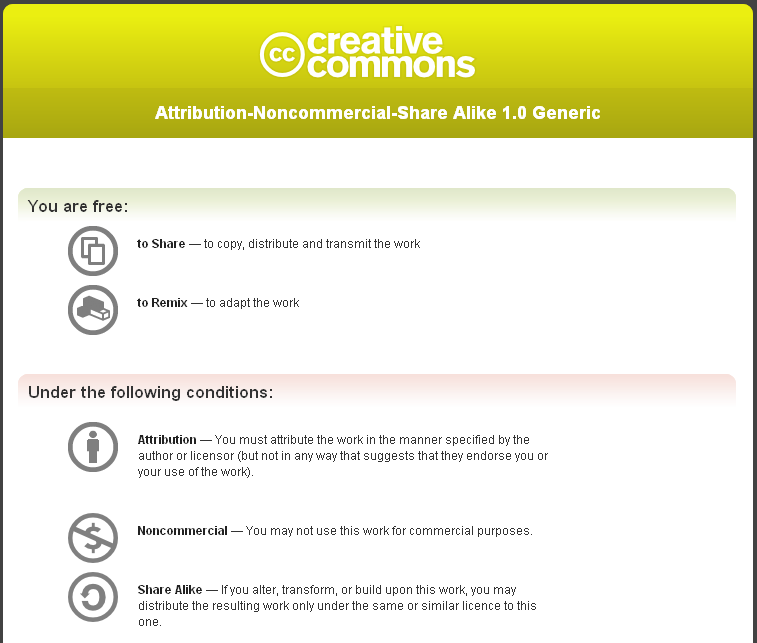
\includegraphics[width=0.50\textwidth]
		{assets/pics/creative_common.png}
	\caption{\license.}
	\label{fig:testGambar}
\end{figure}


%-----------------------------------------------------------------------------%
\section{Membuat Tabel}
%-----------------------------------------------------------------------------%
Seperti pada gambar, tabel juga dapat diberi label dan caption. 
Caption pada tabel terletak pada bagian atas tabel. 
Contoh tabel sederhana dapat dilihat pada \tab~\ref{tab:tab1}.

\begin{table}
	\centering
	\caption{Contoh Tabel}
	\label{tab:tab1}
	\begin{tabular}{| l | c r |}
		\hline
		& kol 1 & kol 2 \\ 
		\hline
		baris 1 & 1 & 2 \\
		baris 2 & 3 & 4 \\
		baris 3 & 5 & 6 \\
		jumlah  & 9 & 12 \\
		\hline
	\end{tabular}
\end{table}

Ada jenis tabel lain yang dapat dibuat dengan \latex~berikut 
beberapa diantaranya. 
Contoh-contoh ini bersumber dari 
\url{http://en.wikibooks.org/wiki/LaTeX/Tables}

\begin{table}
	\centering
	\caption{An Example of Rows Spanning Multiple Columns}
	\label{row.spanning}
	\begin{tabular}{|l|l|*{6}{c|}}
  		\hline % create horizontal line
  		No & Name & \multicolumn{3}{|c|}{Week 1} & \multicolumn{3}{|c|}{Week 2} \\
  		\cline{3-8} % create line from 3rd column till 8th column
  		& & A & B & C & A & B & C\\
  		\hline
  		1 & Lala & 1 & 2 & 3 & 4 & 5 & 6\\
  		2 & Lili & 1 & 2 & 3 & 4 & 5 & 6\\
  		3 & Lulu & 1 & 2 & 3 & 4 & 5 & 6\\
  		\hline
	\end{tabular}
\end{table}

\begin{table}
	\centering
	\caption{An Example of Columns Spanning Multiple Rows}
	\label{column.spanning}
	\begin{tabular}{|l|c|l|}
		\hline
		Percobaan & Iterasi & Waktu \\
		\hline
		Pertama & 1 & 0.1 sec \\ \hline
		\multirow{2}{*}{Kedua} & 1 & 0.1 sec \\
 		& 3 & 0.15 sec \\ 
 		\hline
		\multirow{3}{*}{Ketiga} & 1 & 0.09 sec \\
 		& 2 & 0.16 sec \\
 		& 3 & 0.21 sec \\ 
 		\hline
	\end{tabular}
\end{table}

\begin{table}
	\centering
	\caption{An Example of Spanning in Both Directions Simultaneously}
	\label{mix.spanning}
	\begin{tabular}{cc|c|c|c|c|}
		\cline{3-6}
		& & \multicolumn{4}{|c|}{Title} \\ \cline{3-6}
		& & A & B & C & D \\ \hline
		\multicolumn{1}{|c|}{\multirow{2}{*}{Type}} &
		\multicolumn{1}{|c|}{X} & 1 & 2 & 3 & 4\\ \cline{2-6}
		\multicolumn{1}{|c|}{}                        &
		\multicolumn{1}{|c|}{Y} & 0.5 & 1.0 & 1.5 & 2.0\\ \cline{1-6}
		\multicolumn{1}{|c|}{\multirow{2}{*}{Resource}} &
		\multicolumn{1}{|c|}{I} & 10 & 20 & 30 & 40\\ \cline{2-6}
		\multicolumn{1}{|c|}{}                        &
		\multicolumn{1}{|c|}{J} & 5 & 10 & 15 & 20\\ \cline{1-6}
	\end{tabular}
\end{table}


\chapter{\babTiga}
\label{ch:priorWorks}

This chapter discusses and evaluates the existing benchmarking tools with a set of defined key factors, derived from the requirements.
Section \ref{sec:prior_works.overview} gives an overview of the benchmarking tool considered to be evaluated.
Then in Section \ref{sec:prior_works.method} \first~define the key factors used to evaluate each tools.
Finally, Section \ref{sec:prior_works.evaluation} presents the summary and details of the evaluation of each benchmarking tools.


\section{Overview}
\label{sec:prior_works.overview}

There are five benchmarking tool that \first~selected for evaluation.
This is by no means an exhaustive collection but it should represent the current state of existing benchmarking tools.
\textsc{StarExec} particularly took a web-based approach, where the user submit the configuration and the run happened in the host system.
The rest of them, \textsc{benchmark-tool}, \textsc{BenchExec}, \textsc{BenchKit}, and \textsc{JuBE}, approaches benchmarking as task to be run in the local machine or submitted to a cluster system.


\section{Evaluation method}
\label{sec:prior_works.method}

The requirements from Section \ref{sec:idealBenchmarkingTool} are broken down to a few key factors.
These key factors are used to measure how much of the requirements are fulfilled.

\newcounter{reqCount}
\newcounter{reqFactorCount}[reqCount]
\newcommand{\reqLabel}[1]{
	\setcounter{reqFactorCount}{0}
	\addtocounter{reqCount}{1}
	\arabic{reqCount}.
	#1
}
\newcommand{\reqFactor}[1]{
	\addtocounter{reqFactorCount}{1}
	(\alph{reqFactorCount}) #1
}

\begin{ThreePartTable}
	\begin{TableNotes}
		\footnotesize
		\item[$\alpha$] Subjective evaluation
	\end{TableNotes}
	\begin{longtable}{ll}

		\textbf{Requirements} & \textbf{Factors} \\
		\toprule
		\endhead

		% \cmidrule{2-2}
		\multicolumn{2}{r}{\textit{continued}}
		\endfoot

		\bottomrule
		\insertTableNotes\\
		\caption{Metrics for evaluating existing benchmarking tools}
		\endlastfoot

		\multirow{5}{*}{\reqLabel{Extensibility}}
			& \reqFactor{Flexible evaluation step} \\*
			& \reqFactor{Flexible analysis step} \\*
			& \reqFactor{Flexible benchmark instance source} \\*
			& \reqFactor{Does not enforce implementation type} \\*
			& \reqFactor{Can support arbitrary task scheduler} \\*
		\midrule

		\multirow{5}{*}{\reqLabel{Configurability}}
			& \reqFactor{Multiple runs} \\*
			& \reqFactor{Multiple tool configurations} \\*
			& \reqFactor{Support parameter space} \\*
			& \reqFactor{Benchmark instance selection} \\*
			& \reqFactor{Set resource limit} \\*
		\midrule

		\multirow{5}{*}{\reqLabel{Documentation}}
			& \reqFactor{Self-documenting configuration} \\*
			& \reqFactor{Installation guide} \\*
			& \reqFactor{Configuration guide} \\*
			& \reqFactor{Main workflow guide} \\*
			& \reqFactor{Comprehensive documentation\tnote{$\alpha$}} \\*
		\midrule

		\multirow{4}{*}{\reqLabel{Setup Effort}}
			& \reqFactor{No superuser privilege} \\*
			& \reqFactor{Installation guide} \\*
			& \reqFactor{Documented requirements} \\*
			& \reqFactor{No cumbersome dependencies\tnote{$\alpha$}} \\*
		\midrule

		\multirow{6}{*}{\reqLabel{Accuracy \& Reliability}}
			& \reqFactor{Measure and Limit Resources Accurately} \\*
			& \reqFactor{Terminate Processes Reliably} \\*
			& \reqFactor{Assign Cores Deliberately} \\*
			& \reqFactor{Respect Nonuniform Memory Access} \\*
			& \reqFactor{Avoid Swapping} \\*
			& \reqFactor{Isolate Individual Runs} \\*
		\midrule

		\multirow{5}{*}{\reqLabel{Reproducibility}}
			& \reqFactor{Stored system information} \\*
			& \reqFactor{Sharable results} \\*
			& \reqFactor{Sharable configuration} \\*
			& \reqFactor{Encourage sharable data\tnote{$\alpha$}} \\*
			& \reqFactor{Encourage sharable implementation\tnote{$\alpha$}} \\*
	\end{longtable}
\end{ThreePartTable}

Each of the evaluated tools are scored according to the degree of fulfillment for each requirements.
That is, if $M_i$ is the scored degree of fulfillment of the $i$-th requirement, and $\mu_{i}$ is a vector of size $n$ such that
\[
	\mu_{ij} =
	\begin{cases}
		1 & \text{if the $j$-th key factor of $i$-th requirement is fulfilled}\\
		0 & \text{otherwise}
	\end{cases}
\]
then the degree of fulfillment is the average of $\mu_i$:
\[
	M_i = \frac{\sum\mu_{i}}{|\mu_i|}
\]

Furthermore, as an overall measure, \first~also denote $M_\sigma$ as the overall overage of all $\mu_{i}$ regardless of its requirement category.


\section{Evaluation}
\label{sec:prior_works.evaluation}

\begin{ThreePartTable}
	\begin{TableNotes}
		\footnotesize
		\item[*] Values are emptied if it's not applicable. The complete evaluation is given in the appendix.
	\end{TableNotes}
	\begin{longtable}{lddddddd}
		& \multicolumn{1}{c}{$M_1$} & \multicolumn{1}{c}{$M_2$} & \multicolumn{1}{c}{$M_3$} & \multicolumn{1}{c}{$M_4$} & \multicolumn{1}{c}{$M_5$} & \multicolumn{1}{c}{$M_6$} & \multicolumn{1}{c}{$M_\sigma$}\\
		\midrule
		\textsc{benchmark-tool} & .60 & .80 & .20 & .50 & .17 & .40 & .43 \\
		\textsc{BenchExec} & .40 & .60 & .60 & .50 & 1.00 & .80 & .66 \\
		\textsc{Benchkit} & .40 & .40 & .60 & .25 & .50 & .40 & .43 \\
		\textsc{JuBE} & .80 & 1.00 & 1.00 & 1.00 & & .40 & .83 \\
		% \textsc{Optil.io} & .40 & .80 & .60 & 1.00 & & .40 & .62 \\
		\textsc{StarExec} & .60 & .60 & .80 & 1.00 & 1.00 & 1.00 & .83 \\
		\bottomrule
		\insertTableNotes\\
		\caption{Requirements score for various existing benchmarking tools}
		\label{tab:reqscoresummary}
	\end{longtable}
\end{ThreePartTable}

Table \ref{tab:reqscoresummary} shows that none of the considered benchmarking tools fulfilled the requirements given.
The closest is \textsc{StarExec} and \textsc{JuBE}.
\textsc{StarExec} can even---arguably---achieves $\bm{R_1}$ by default.
But most of the features available in \textsc{StarExec}, such as managing post-processors and plots, are restricted to the community leaders.
The normal user is forced to use what was already available in the community space.
On the other hand, \textsc{JuBE} is too generic and provides little support for reproducibility.

Further descriptions and evaluations of each benchmarking tools are given below.

\subsection{\textsc{benchmark-tool}}
\textsc{benchmark-tool}\footnote{\href{https://github.com/potassco/benchmark-tool}{https://github.com/potassco/benchmark-tool}} is originally a part of Potassco\footnote{\href{https://potassco.org/}{https://potassco.org/}}, the Postdam Answer Set Solving Collection, developed at the University of Potsdam.
It has been forked and used by some researchers in the computational logic field, such as its use in Technicsche Universität Dresden and Technicsche Universität Wien.

The general workflow is like this:
(a) create a \textit{runscript}, defining the benchmark run configuration;
(b) generate the file necessary for the benchmark by running the \code{bgen} script;
(c) run the benchmark by running the script generated in the output dir;
(d) evaluate the benchmark by running the \code{beval} script, outputting an xml file;
(e) generate a CSV or OpenOffice spreadsheet from the evaluated result by running the \code{bconv} script.

This benchmarking tool is not designed to be reusable.
Instead, the user has to clone the source code, then add their benchmarking config on top of the cloned code.
This makes it possible to achieve some degree of extensibility.
For example, it can be extended to submit the benchmarking job to any cluster job scheduler, like Slurm or HTCondor by writing a specific script generation used in the step (b).
On the other hand, this also makes it hard to share the configuration without actually sharing the whole cloned source code.
Some user even uses a centralized git repository and manages different benchmarks with git branches.

This tool is also lacking in documentation and accuracy.
The only documentation available is minimal and not has not been updated since 9 years ago.
Additionally, it uses \textsc{runsolver} to measure and limit the resources.
According to \citet{beyerReliableBenchmarkingRequirements2019}, \textsc{runsolver} is not accurate and reliable.

Setting up a benchmark with this tool takes a lot effort.
The requirements for the Python interpreter and external requirements is not made clear in the 9 years old documentation.
There is also certain rules for location and name of the tool that will be used.
Furthermore, writing the \textit{result parser} often involves a lot of copying since there is no certain definition of it and most of the time it is specific to each benchmark.

\First~tried to refactor this tool to some degree\footnote{\href{https://github.com/daajoe/benchmark-tool/tree/refactor}{https://github.com/daajoe/benchmark-tool/tree/refactor}}, but decided to create a new tool instead in the middle of refactoring.
This is because to create the ideal tool, we need significant architecture overhaul and decided it's better to start anew.

\subsection{\textsc{BenchExec}}

\textsc{BenchExec} \citep{philipp_wendler_2019_2561835} is developed by the Software and Computational Systems Lab of Ludwig-Maximilians-Universität München (LMU Munich)\footnote{\href{https://www.sosy-lab.org/}{https://www.sosy-lab.org/}} with the main goal of reliable measurement and limitation of resource usage.
It has been used successfully and proven its reliability and usefulness in the International Competition on Software Verification (SV-COMP) \citep{beyerReliableBenchmarkingRequirements2019}.
It is actively developed with the last release (as of 24th April 2019) in 11th February 2019 and licensed under the Apache License 2.0.

To achieve accuracy and reliability, they developed a new resource usage measurement and limiting tool, \textsc{RunExec}.
This tool uses linux-specific features, Linux Control Groups (CGroup) and Linux Containers optionally.
This allows the tool to contain the underlying process and its descendants reliably to then measure their accumulated resource usage accurately.
But in turn this also makes the installation a bit difficult and requires a minimum requirement for the kernel (full support for these features is available in Linux kernel 3.18 onwards).
Setting up CGroups in particular requires superuser access which often is not directly available in shared cluster systems.

The general workflow for benchmarking with this tool is as follows:
(a) defining an xml configuration file for the benchmark;
(b) defining a tasks set to be run (optionally in a yaml definition);
(c) reusing or defining a new \textit{tool-info module} for the tool to benchmark;
(d) running the \code{benchexec} program with the xml configuration;
(e) generating interactive table and plots with the \code{table-generator} program.

The documentation for this benchmarking framework, although somewhat sufficient, is not comprehensive and feels incomplete.
There is no tutorial or guides for getting started on benchmarking, instead the documentation revolves around the usage of each tools.
This makes following the documentation a bit difficult because the information is scattered across files.

The modular structure of this framework makes it extensible.
Tools are defined in self-contained \textit{tool-info modules} and can be reused.
They encourage user to submit a pull request for their \textit{tool-info modules} to the main repository so other user can reuse it, albeit this does not mean that the tool itself is made available to achieve $\bm{R_1}$.
There is also an executor module that can be written to enable running the benchmark in arbitrary execution environment, such as in cluster system.

\begin{listing}
	\begin{minted}{text}
		CHECK( init(main()), LTL(G valid-free) )
		CHECK( init(main()), LTL(G valid-deref) )
		CHECK( init(main()), LTL(G valid-memtrack) )
	\end{minted}
	\caption{An example property definition for \textsc{BenchExec}}
	\label{lst:benchexec.property}
\end{listing}

The downside of this framework is the evaluation is tightly coupled to the convention used in SV-COMP.
They use a property file like the one listed in Listing \ref{lst:benchexec.property}, specific to the competition.
Combined with the lack of documentation, this makes it impossible, for now, to evaluate and analyze a benchmark outside the scope of software verification with \textsc{BenchExec}.


\subsection{\textsc{Benchkit}}

\textsc{Benchkit} \citep{benchkit:2013} is a benchmarking tool actively used in the Model Checking Contest (MCC)\footnote{\href{https://mcc.lip6.fr/}{https://mcc.lip6.fr/}}.
The competition participants submit a virtual machine consisting of the (minimal) operating system (OS) to run the program, dependencies, and a small \textsc{BenchKit} head to interface with the \textsc{BenchKit} kernel.

The documentation for this tool\footnote{\href{http://cosyverif.org/wp-content/benchmarks/BenchKit.pdf}{http://cosyverif.org/wp-content/benchmarks/BenchKit.pdf}} has not been updated since version $\beta1$, released in February, 2013.
This documentation is plentiful and guides the user through the general workflow, but the workflow itself is confusing to follow.

This tool allows the user to run the benchmark across remote nodes, which in turn execute the run inside multiple virtual machines (this is not yet the case in the $\beta1$ version of the software described in the documentation).
The result is then compiled manually or sent automatically through e-mails from the remote nodes and then manually analyzed from the generated CSV files.
It also forces certain requirements before running the benchmarks, such as the need for a specific folder structure, and the deployment of virtual machine images to the remote nodes in advance.

It uses \textsc{SysStat}\footnote{\href{https://github.com/sysstat/sysstat}{https://github.com/sysstat/sysstat}}, which measures the whole virtual machine resource usage.
This means that the resource usage measured also includes the OS.
Accordingly, \cite{beyerReliableBenchmarkingRequirements2019} assess this measurement tool as neither accurate nor reliable.

Although the necessity of providing virtual machine makes sure the program is $\bm{R_1}$ reproducible, \citet{kordonBenchKitToolMassive2014} reported an overhead of 40 seconds per run in their experiment due to the boot-up time of virtual machines.
\cite{beyerReliableBenchmarkingRequirements2019} remarks that this 40 seconds overhead would have taken an additional 190 CPU days if used in their competition, definitely a prohibitive overhead.


\subsection{\textsc{JuBE}}

\textsc{JuBE} \citep{frings2010flexible} is a benchmarking environment developed by Jülich Supercomputing Centre (JSC) of Forschungszentrum Jülich, Germany.
It is actively developed, albeit with no public version control repository, with the last release (as of 24th April 2019) in 4th February 2019.
It is licensed under the GNU General Public License version 3.

Compared to other benchmarking tool, it approaches the benchmarking task in a different, completely generic way.
There is no explicit measurement and limiter tool, no explicit task instances, and no specific evaluation or analysis step.
Instead, all the benchmarking task revolves around steps, parameters, and pattern-based analyzers.

The parameters can be defined as static, a parameter space, or even dynamic parameter space with the help scripting languages such as Python.
The steps are just a shell command, receiving several variables from the parameters and \textsc{JuBE} itself.
Finally, the analyzer just match patterns to the files generated from the benchmarking steps, then produce a CSV file.

The documentation\footnote{\href{https://apps.fz-juelich.de/jsc/jube/jube2/docu/index.html}{https://apps.fz-juelich.de/jsc/jube/jube2/docu/index.html}} is comprehensive and checks all the marks in \firstposs~$M_3$ evaluation.
There is a quick start guide and various advanced usage guides available.
Every command also has all its options documented.

Since it has no preference of resource measurement and limiter tool, \first~can't evaluate $M_5$.
But it definitely has the potential to use any kind of tool to measure and limit the resource usage.
This is also the case for the execution environment.
Submitting the benchmarking task to a job queue is just another benchmarking step.

The flexibility of this tool is surely its strong point.
But this flexibility also burdens the user to do all the repetitive task of benchmarking on their own, although it is possible to create some reusable wrappers for these repetitive tasks.
The analysis step is also restricting, since the user has to output the metrics to a file, then capture it with patterns.
Additionally, the tool itself does not provide much in terms of reproducibility.
It is up to the user how to make their benchmarking reproducible since shell commands is often not reproducible by itself.


\subsection{\textsc{StarExec}}

\textsc{StarExec} is a web-based service for evaluating logic solvers on user-supplied benchmarks input \citep{stumpStarExecCrossCommunityInfrastructure2014}.
It is officially hosted at \href{https://www.starexec.org/}{\code{https://www.starexec.org/}}.
The source code is publicly available\footnote{\href{https://github.com/StarExec/StarExec}{https://github.com/StarExec/StarExec}} and is actively developed under the MIT license.
\First~will consider the hosted version of this tool for the evaluation.

The service is built around the ideas of \emph{spaces} and \emph{primitives}.
A space is a collection of solvers, benchmarks, jobs, and users, collectively defined as \emph{primitives}.
Spaces have a hierarchical structure.
The topmost spaces are called the \emph{community spaces}, while the descendants are called \emph{subspaces} \citep{stumpStarExecCrossCommunityInfrastructure2014}.

The documentation for this service is by no mean complete, but it is detailed enough for a normal user.
Measurement and limitation of resource usage currently can be handled by either \textsc{runsolver} or \textsc{RunExec} from \textsc{BenchExec}.
There is also an active effort to apply containerization feature of \textsc{RunExec}.

To register, a user has to apply to be approved---or in other words, endorsed---by a community leader, the person managing a community space.
Then after accepted, the user can log in and view the public spaces in their community or create new subspaces.
Users can submit their own solvers and benchmarks to a space, which can also be copied across spaces.
A benchmarking job can then be submitted with the existing solver configurations, benchmarks, and predetermined post-processors.
These community-specific post-processors can only be configured by a community leader.

The service encourage shared solvers and benchmarks in the community to reduce duplication of effort.
This also helps the community practice $\bm{R_1}$ reproducibility.
Other users can re-run another user's job to confirm the results in a fully reproducible way since the execution environment is the same.

The limitation that only the community leaders can approve members and configure things like pre- and post-processors is limiting the capability of this service.
Sure, for a specific community the measured metrics is more or less the same, but this also prevent other metrics to be evaluated freely.
This decision might be necessary to prevent abuse as this involves sharing a large computing power.
\chapter{\babEmpat}

\section{Overview}

To objectively compare two or more programs, an objective measurement is needed.
Resource consumption like CPU time elapsed, CPU instruction used, or peak memory usage is often considered as the go-to measurement for benchmarking in computational science.
The resources measured might include information regarding processes, threads, computation, memory, input/output, and files of a program \citep{juvePracticalResourceMonitoring2015}.

The measurement of these resource consumption is not only used in benchmarking.
Some of its usage includes but not limited to:
its daily usage in user program such as \textit{Task Manager} in Windows or \code{top} in Linux,
judging whether a program passes some threshold marks in education or competition field,
measuring the efficiency of a job scheduling system in High Throughput Computing (HTC) field [need citation],
selecting dataset for a competition,
and getting best-enough result from an iterative optimization algorithm after some desired time.
Because of this wide area of usage, there are many attempts to implement these measurement to achieve the best result.

\section{Monitoring Mechanism}

\citet{juvePracticalResourceMonitoring2015} distinguish resource monitoring into three different mechanism.
There are tradeoffs between these mechanisms and so it's often preferred to use a combination of more than one mechanism to achieve better results.

\subsection{Query}

The query approach works by querying resource usage information directly from the operating system.
To monitor the resource usage over time, this means the query is executed at some interval, effectively doing a polling mechanism.
More frequent polling will result in a more timely information but the overhead also increases.
Querying is often the easiest resource monitoring mechanism in term of implementation \citep{juvePracticalResourceMonitoring2015}.

It is the least intrusive mechanism, albeit the information received from this mechanism also immediately expires.
A resource usage surge could happen in between the queries, so this mechanism is not accurate.
In short, the query mechanism provides an easy to implement but inaccurate measurement of the resource monitored.

\code{getrusage()}\footnote{see \href{https://linux.die.net/man/2/getrusage}{\code{man getrusage}}} is a POSIX standard system call.
Unfortunately, this standard only specifies \code{ru\_utime} and \code{ru\_stime}, the user mode time spent and kernel mode time spent, respectively.
In practice, \code{getrusage()} includes more information, for example the \code{ru\_maxrss}, indicating the maximum resident set size.

A Linux specific feature that is often used for querying resource usage is the procfs\footnote{see \href{https://linux.die.net/man/5/proc}{\code{man 5 proc}}} pseudo-file system.
The information provided includes user time, system time, resident set size, number of threads, and many more.
On a side note, since the operating system always account these informations for all running processes, the clock resolution used is not too accurate.
The user time and system time in \code{/proc/[pid]/stat} is measured in system ticks, which turns out to be 10 milliseconds in a typical Linux system.
Recently, Linux control groups (CGroups)\footnote{see \href{http://man7.org/linux/man-pages/man7/cgroups.7.html}{\code{man 7 cgroups}}} is also used for querying similar or more comprehensive information for a group of processes.

A more universal query mechanism is using performance counters.
Most system nowadays---disregarding its operating system---has a hardware clock that has an incredibly accurate clock resolution, some even achieving nanoseconds resolution.
Querying this clock at the start and end of a program could measure what is called the wall clock time.
This measurement is less informative than CPU times measured by user time and system time, but still useful in spite of that.

The library \code{psutil}\footnote{\href{https://github.com/giampaolo/psutil}{https://github.com/giampaolo/psutil}} provides an abstraction for various resource queries that works in many operating systems.
This allows a cross-platform resource monitoring tool based on query mechanism to be developed.
As of now however, \first~can't find the relevant resource monitoring tool making use of this abstraction.

It is also need to be noted that this query mechanism cannot work with process tree reliably.
Because of the nature of polling, short living processes can be missed and not accounted to the final result.
This is a strong restriction because most of the computation in HTC or computational science in general often make use of parallelism or concurrency.


\subsection{Notification}

A more reliable mechanism to query a resource usage is to ask the system itself to report the usage on specific events.
This also produces less overhead compared to the query mechanism, although the information queried also immediately expires \citep{juvePracticalResourceMonitoring2015}.

\code{wait4()}\footnote{see \href{https://linux.die.net/man/2/wait4}{\code{man wait4}}} is a system call available in most UNIX that waits for a child process (and blocks the process calling this system call), then returns its \code{getrusage()} information when the process exits.
This one example of the notification mechanism in practice.

\code{inotify}\footnote{see \href{https://linux.die.net/man/7/inotify}{\code{man inotify}}} application programming interface (API) in Linux can also be leveraged.
This API allows one to listen for file system events, such as new file or directory created, existing files edited, a file is accessed, or a file is deleted.
Most operating system also have APIs similar to this, such as \code{fsevents} in OS X. Watchman\footnote{\href{https://facebook.github.io/watchman/}{https://facebook.github.io/watchman/}} is an open source tool by Facebook that abstracts these file system notification APIs.

Another useful notification is \code{forkstat}\footnote{\href{http://manpages.ubuntu.com/manpages/cosmic/en/man8/forkstat.8.html}{http://manpages.ubuntu.com/manpages/cosmic/en/man8/forkstat.8.html}}.
This tool notify system-wide \code{fork()}, \code{exec()}, and \code{exit()} system call activities.
Unfortunately, this tool needs superuser privilege because uses Linux netlink connector, a special socket for communication between kernel and user space.

A more powerful albeit intrusive notification can be achieved by using the UNIX \code{ptrace()}\footnote{see \href{https://linux.die.net/man/2/ptrace}{\code{man ptrace}}} system call.
\code{ptrace()}, often use for debugging, allows a process to intercept and modify system calls.
When a system call occurs, the kernel will check if the process is being traced, and if so, will notify the tracer.
With this system call one can observe, for example, the \code{fork()}, \code{exec()}, and \code{exit()} system call to track process trees.

Combining this notifications with the earlier query mechanism can result in a more powerful resource monitoring method.
For example, one can watch for filesystem events on a specific part of the filesystem, such as the \code{/tmp}, \code{/var}, or a specific work directory of the running application. Then when an event occurs, a procfs query is executed to catch the short-living process causing the event is executed.
This effectively allows the procfs query method to work more reliably compared to blindly polling the pseudo-file system.

\subsection{Interposition}

\citet{juvePracticalResourceMonitoring2015} defines this group of mechanism as the ones in which the monitor intercepts actions performed by the process.
This mechanism is highly intrusive because it actively changes the way the program runs.
\code{ptrace()} mentioned earlier also belongs to this group since the kernel stops the system call and forward an event to the monitor (in this case the tracer).
In general this method introduces huge overhead compared to the other mechanism.
In \code{ptrace()} for example, there need to be at least two context switches for every system call intercepted.

A less intrusive method compared to the one \code{ptrace()} used is function interposition.
In this mechanism, the monitor replace some original function by a wrapper that also record parameters and results of the original function \citep{juvePracticalResourceMonitoring2015}.
The environment variable \code{LD\_PRELOAD} in Linux and \code{DYLD\_INSERT\_LIBRARIES} in OS X provides an easy way to load arbitrary library before running a dynamically-linked program.
This way, one can write a wrapper function that will be called instead of the original function.

On the other hand, \code{ptrace()} is less practical because it interrupts each system call made by the program, but it is more robust and can be used in statically-linked programs.
\citet{kimPracticalEffectiveSandboxing2013} has shown that using the recent \code{seccomp/BPF}\footnote{see \href{http://man7.org/linux/man-pages/man2/seccomp.2.html}{\code{man seccomp}}} feature to filter out what system call is going to be intercepted results in an efficient system call interposition technique.

\code{seccomp} is a security feature in Linux (since 2.6.23) to allow only some set of system calls for a program.
Furthermore, Berkeley Packet Filter (\code{BPF}) is also supported since Linux 3.5 as a mean to configure the way \code{seccomp} filters the system call.
With the combination of \code{seccomp} and \code{BPF}, they can configure only some set of the system call to send a \code{ptrace()} event while the rest just continue normally, effectively reducing the overhead of system call interposition.
This feature---usually combined with Linux namespaces---can also be used to provide simple yet secure isolation for the program, as used by \textsc{nsjail}\footnote{see Section \ref{sec:resource.impl.nsjail}} and \textsc{firejail}\footnote{\href{https://github.com/netblue30/firejail/}{https://github.com/netblue30/firejail/}}.

With this interposition mechanism, one can reliably use the query mechanism.
For example, before the \code{exit()} system call actually happen, the \code{procfs} can be queried because the program itself can be stopped before the entry is removed from the pseudo-file system.
While this is the most accurate method compared to the others, this is also highly intrusive so caution must be exercised when using this method.

\section{Virtualization: More Reliable Measurements}

To strengthen the need to produce more reliable resource usage measurement, \citet{beyerReliableBenchmarkingRequirements2019} states isolation of runs as one of the requirements for an accurate and reliable benchmarking.
Specifically, they used Linux containers to provide a lightweight isolation.
Additionally, virtualization tools that are widely used also contributes to reproducibility by providing a programmatic way to pack program dependencies \citep{boettigerIntroductionDockerReproducible2015,kordonBenchKitToolMassive2014:2013}.

\subsection{Virtual Machines}

Virtual machines (VMs) use a technique called hypervisor-based virtualization.
Hypervisor is a software that creates and runs virtual machines \citep{scheepersVirtualizationContainerizationApplication2014}.
There are many of such hypervisor programs that are widely used, examples includes VirtualBox, Xen, Hyper-V, and many more.

Hypervisor manages the resource that will be used by the VMs.
When deployed, each VM run its own operating system with its own kernel.
All the dependencies needed by the program, is also included in the VM itself.
This results in a portable and isolated way to run a program.

Alas, this comprehensive virtualization comes with a cost.
The overhead of bootstrapping a VM is not negligible.
\citet{kordonBenchKitToolMassive2014} reports an average of 40 seconds of booting overhead when this virtualization is used in benchmarking.
\citet{scheepersVirtualizationContainerizationApplication2014} recommends using VMs (compared to containers) when it is important to distribute resources equally and performance should be less dependent from other running tasks.

\subsection{Containers}

A relatively new technique addressing the overhead issue is container-based virtualization.
Linux Containers (LXC)\footnote{\href{https://linuxcontainers.org/}{https://linuxcontainers.org/}} uses this technique to create an isolated environment without hosting multiple kernels like in hypervisor-based virtualization.
The implementation share the Linux kernel with the host machine.
This makes it more lightweight and particularly good for deploying many small isolated instances, as often the case in benchmarking.

Docker\footnote{\href{https://www.docker.com/}{https://www.docker.com/}} is an especially popular tool that utilizes LXC and offer an easy to use interface.
An application built with Docker extends upon existing Docker images with a reproducible \code{Dockerfile} configuration, stating each step needed to create the exact image.
With the key feature of sharing the Linux kernel, an OS image in Docker can achieve minimum size, with a notable example like Alpine Linux even reaching only 2-3 megabytes in size (its virtual machine images is ten times larger in size).

\citet{zhangComparativeStudyContainers2018} report a much less boot up latency---period from starting a VM or container to usable service---in Docker containers compared to VMs.
Booting a VM when there are about 250 other idle VMs takes more than 1000 seconds, while booting 512 Docker contains only takes 987 seconds (an average of 1.89 seconds per container).
This is also true for the amount of memory consumed in idle state.
A VM takes 0.23 GB compared to 0.03 GB of memory of Docker container in their experiment.

\section{Implementations}

We consider some existing implementation and discuss their method of measuring and limiting resource.

\subsection{\textsc{runsolver}}

\subsection{\textsc{runexec}}

\subsection{\textsc{kickstart}}

\subsection{\textsc{timeout}}

\subsection{\textsc{nsjail}}
\label{sec:resource.impl.nsjail}

\subsection{\textsc{isolate}}

\subsection{\textsc{psmon}}
%-----------------------------------------------------------------------------%
\chapter{\babLima}
%-----------------------------------------------------------------------------%
\todo{Tambahkan kata-kata pengantar bab 5 disini.}


%-----------------------------------------------------------------------------%
\section{Mengubah Tampilan Teks}
%-----------------------------------------------------------------------------%
Beberapa perintah yang dapat digunakan untuk mengubah tampilan adalah: 
\begin{itemize}
	\item \bslash f \\
		Merupakan alias untuk perintah \bslash textit, contoh 
		\f{contoh hasil tulisan}.
	\item \bslash bi \\
		\bi{Contoh hasil tulisan}.
	\item \bslash bo \\
		\bo{Contoh hasil tulisan}.
	\item \bslash m \\
		Contoh\ hasil\ tulisan: $\alpha \not= \m{\alpha}$
	\item \bslash code \\ 
		\code{Contoh hasil tulisan}.
\end{itemize}


%-----------------------------------------------------------------------------%
\section{Memberikan Catatan}
%-----------------------------------------------------------------------------%
Ada dua perintah untuk memberikan catatan penulisan dalam dokumen yang Anda 
kerjakan, yaitu: 
\begin{itemize}
	\item \bslash todo \\
		Contoh: \\ \todo{Contoh bentuk todo.}
	\item \bslash todoCite \\ 
		Contoh: \todoCite
\end{itemize}


%-----------------------------------------------------------------------------%
\section{Menambah Isi Daftar Isi}
%-----------------------------------------------------------------------------%
Terkadang ada kebutuhan untuk memasukan kata-kata tertentu kedalam Daftar Isi. 
Perintah \bslash addChapter dapat digunakan untuk judul bab dalam Daftar isi. 
Contohnya dapat dilihat pada berkas thesis.tex.


%-----------------------------------------------------------------------------%
\section{Memasukan PDF}
%-----------------------------------------------------------------------------%
Untuk memasukan PDF dapat menggunakan perintah \bslash inpdf yang menerima satu 
buah argumen. Argumen ini berisi nama berkas yang akan digabungkan dalam 
laporan. PDF yang dimasukan degnan cara ini akan memiliki header dan footer 
seperti pada halaman lainnya. 

\inpdf{assets/pdfs/include}

Cara lain untuk memasukan PDF adalah dengan menggunakan perintah \bslash putpdf 
dengan satu argumen yang berisi nama berkas pdf. Berbeda dengan perintah 
sebelumnya, PDF yang dimasukan dengan cara ini tidak akan memiliki footer atau 
header seperti pada halaman lainnya. 

\putpdf{assets/pdfs/include}


%-----------------------------------------------------------------------------%
\section{Membuat Perintah Baru}
%-----------------------------------------------------------------------------%
Ada dua perintah yang dapat digunakan untuk membuat perintah baru, yaitu: 
\begin{itemize}
	\item \bslash Var \\
		Digunakan untuk membuat perintah baru, namun setiap kata yang diberikan
		akan diproses dahulu menjadi huruf kapital. 
		Contoh jika perintahnya adalah \bslash Var\{adalah\} makan ketika 
		perintah \bslash Var dipanggil, yang akan muncul adalah ADALAH. 
	\item \bslash var \\
		Digunakan untuk membuat perintah atau baru. 
\end{itemize}


%-----------------------------------------------------------------------------%
\chapter{\babEnam}
%-----------------------------------------------------------------------------%
\todo{tambahkan kata-kata pengantar bab 6 disini}


%---------------------------------------------------------------
\chapter{\kesimpulan}
%---------------------------------------------------------------
\todo{Tambahkan kesimpulan dan saran terkait dengan perkerjaan 
	yang dilakukan.}


%---------------------------------------------------------------
\section{Kesimpulan}
%---------------------------------------------------------------


%---------------------------------------------------------------
\section{Saran}
%---------------------------------------------------------------


%
% Daftar Pustaka
%\input{pustaka}

% Alternatif manajemen daftar pustaka dengan \bibliography
\bibliographystyle{apalike}
\bibliography{pustaka}

%
% Lampiran 
%
% \begin{appendix}
% 	%
% @author  Andreas Febrian
% @version 1.00 
% 
% Hanya sebuah pembatas bertuliskan LAMPIRAN ditengah halaman. 
% 

\begin{titlepage}
	\centering 
	\vspace*{6cm}
	\noindent \Huge{APPENDIX}
	\addChapter{APPENDIX}
\end{titlepage}
% 	\setcounter{page}{2}\textbf{}
% 	%-----------------------------------------------------------------------------%
\addChapter{Appendix 1}
\chapter*{Appendix 1: Source Code}
%-----------------------------------------------------------------------------%

% \captionof*{listing}{examples/sat/sat/validate.py}
% \inputminted{python}{assets/listings/reprobench/examples/sat/sat/validate.py}
% \captionof*{listing}{examples/sat/tools/\_\_init\_\_.py}
% \inputminted{python}{assets/listings/reprobench/examples/sat/tools/__init__.py}
% \captionof*{listing}{examples/sat/tools/glucose.py}
% \inputminted{python}{assets/listings/reprobench/examples/sat/tools/glucose.py}
% \captionof*{listing}{examples/sat/tools/lingeling.py}
% \inputminted{python}{assets/listings/reprobench/examples/sat/tools/lingeling.py}
% \captionof*{listing}{examples/sudokusat/sudoku/validate.py}
% \inputminted{python}{assets/listings/reprobench/examples/sudokusat/sudoku/validate.py}
% \captionof*{listing}{examples/sudokusat/tools/\_\_init\_\_.py}
% \inputminted{python}{assets/listings/reprobench/examples/sudokusat/tools/__init__.py}
% \captionof*{listing}{examples/sudokusat/tools/sudoku\_team1.py}
% \inputminted{python}{assets/listings/reprobench/examples/sudokusat/tools/sudoku_team1.py}

% \captionof*{listing}{reprobench/\_\_init\_\_.py}
% \inputminted{python}{assets/listings/reprobench/reprobench/__init__.py}


% \captionof*{listing}{reprobench/console/decorators.py}
% \inputminted{python}{assets/listings/reprobench/reprobench/console/decorators.py}

\captionof*{listing}{reprobench/console/main.py}
\inputminted{python}{assets/listings/reprobench/reprobench/console/main.py}

\captionof*{listing}{reprobench/console/status.py}
\inputminted{python}{assets/listings/reprobench/reprobench/console/status.py}

\captionof*{listing}{reprobench/core/analyzer.py}
\inputminted{python}{assets/listings/reprobench/reprobench/core/analyzer.py}

\captionof*{listing}{reprobench/core/base.py}
\inputminted{python}{assets/listings/reprobench/reprobench/core/base.py}

% \captionof*{listing}{reprobench/core/bootstrap/\_\_init\_\_.py}
% \inputminted{python}{assets/listings/reprobench/reprobench/core/bootstrap/__init__.py}

\captionof*{listing}{reprobench/core/bootstrap/client.py}
\inputminted{python}{assets/listings/reprobench/reprobench/core/bootstrap/client.py}

\captionof*{listing}{reprobench/core/bootstrap/server.py}
\inputminted{python}{assets/listings/reprobench/reprobench/core/bootstrap/server.py}

\captionof*{listing}{reprobench/core/db.py}
\inputminted{python}{assets/listings/reprobench/reprobench/core/db.py}

% \captionof*{listing}{reprobench/core/events.py}
% \inputminted{python}{assets/listings/reprobench/reprobench/core/events.py}

% \captionof*{listing}{reprobench/core/exceptions.py}
% \inputminted{python}{assets/listings/reprobench/reprobench/core/exceptions.py}

\captionof*{listing}{reprobench/core/observers.py}
\inputminted{python}{assets/listings/reprobench/reprobench/core/observers.py}

\captionof*{listing}{reprobench/core/schema.py}
\inputminted{python}{assets/listings/reprobench/reprobench/core/schema.py}

\captionof*{listing}{reprobench/core/server.py}
\inputminted{python}{assets/listings/reprobench/reprobench/core/server.py}

\captionof*{listing}{reprobench/core/sysinfo.py}
\inputminted{python}{assets/listings/reprobench/reprobench/core/sysinfo.py}

\captionof*{listing}{reprobench/core/worker.py}
\inputminted{python}{assets/listings/reprobench/reprobench/core/worker.py}

% \captionof*{listing}{reprobench/executors/\_\_init\_\_.py}
% \inputminted{python}{assets/listings/reprobench/reprobench/executors/__init__.py}

\captionof*{listing}{reprobench/executors/base.py}
\inputminted{python}{assets/listings/reprobench/reprobench/executors/base.py}

\captionof*{listing}{reprobench/executors/db.py}
\inputminted{python}{assets/listings/reprobench/reprobench/executors/db.py}

% \captionof*{listing}{reprobench/executors/events.py}
% \inputminted{python}{assets/listings/reprobench/reprobench/executors/events.py}

\captionof*{listing}{reprobench/executors/psmon.py}
\inputminted{python}{assets/listings/reprobench/reprobench/executors/psmon.py}

% \captionof*{listing}{reprobench/managers/\_\_init\_\_.py}
% \inputminted{python}{assets/listings/reprobench/reprobench/managers/__init__.py}

\captionof*{listing}{reprobench/managers/base.py}
\inputminted{python}{assets/listings/reprobench/reprobench/managers/base.py}

\captionof*{listing}{reprobench/managers/local/\_\_init\_\_.py}
\inputminted{python}{assets/listings/reprobench/reprobench/managers/local/__init__.py}

\captionof*{listing}{reprobench/managers/local/manager.py}
\inputminted{python}{assets/listings/reprobench/reprobench/managers/local/manager.py}

\captionof*{listing}{reprobench/managers/slurm/\_\_init\_\_.py}
\inputminted{python}{assets/listings/reprobench/reprobench/managers/slurm/__init__.py}

\captionof*{listing}{reprobench/managers/slurm/manager.py}
\inputminted{python}{assets/listings/reprobench/reprobench/managers/slurm/manager.py}

% \captionof*{listing}{reprobench/managers/slurm/utils.py}
% \inputminted{python}{assets/listings/reprobench/reprobench/managers/slurm/utils.py}

% \captionof*{listing}{reprobench/statistics/plots/\_\_init\_\_.py}
% \inputminted{python}{assets/listings/reprobench/reprobench/statistics/plots/__init__.py}

\captionof*{listing}{reprobench/statistics/plots/base.py}
\inputminted{python}{assets/listings/reprobench/reprobench/statistics/plots/base.py}

\captionof*{listing}{reprobench/statistics/plots/cactus/\_\_init\_\_.py}
\inputminted{python}{assets/listings/reprobench/reprobench/statistics/plots/cactus/__init__.py}

% \captionof*{listing}{reprobench/statistics/plots/cactus/template.ipynb}
% \inputminted{python}{assets/listings/reprobench/reprobench/statistics/plots/cactus/template.ipynb}

% \captionof*{listing}{reprobench/statistics/tables/\_\_init\_\_.py}
% \inputminted{python}{assets/listings/reprobench/reprobench/statistics/tables/__init__.py}

\captionof*{listing}{reprobench/statistics/tables/base.py}
\inputminted{python}{assets/listings/reprobench/reprobench/statistics/tables/base.py}

\captionof*{listing}{reprobench/statistics/tables/run.py}
\inputminted{python}{assets/listings/reprobench/reprobench/statistics/tables/run.py}

% \captionof*{listing}{reprobench/task\_sources/base.py}
% \inputminted{python}{assets/listings/reprobench/reprobench/task_sources/base.py}

\captionof*{listing}{reprobench/task\_sources/doi/\_\_init\_\_.py}
\inputminted{python}{assets/listings/reprobench/reprobench/task_sources/doi/__init__.py}

% \captionof*{listing}{reprobench/task\_sources/doi/base.py}
% \inputminted{python}{assets/listings/reprobench/reprobench/task_sources/doi/base.py}

\captionof*{listing}{reprobench/task\_sources/doi/zenodo.py}
\inputminted{python}{assets/listings/reprobench/reprobench/task_sources/doi/zenodo.py}

\captionof*{listing}{reprobench/task\_sources/file.py}
\inputminted{python}{assets/listings/reprobench/reprobench/task_sources/file.py}

\captionof*{listing}{reprobench/task\_sources/url.py}
\inputminted{python}{assets/listings/reprobench/reprobench/task_sources/url.py}

\captionof*{listing}{reprobench/tools/executable.py}
\inputminted{python}{assets/listings/reprobench/reprobench/tools/executable.py}

% \captionof*{listing}{reprobench/utils.py}
% \inputminted{python}{assets/listings/reprobench/reprobench/utils.py}
% \end{appendix}

\end{document}